\documentclass[12pt, a4paper, twoside]{book}
\usepackage[utf8]{inputenc}
\usepackage[english, serbianc]{babel}
\usepackage{lipsum}
\usepackage{graphicx}
\usepackage{multicol}
\usepackage{booktabs}
\usepackage{float}

\usepackage{geometry}
\geometry{
	a4paper,
	total={160mm,237mm},
	left=30mm,
	top=30mm,
}

\usepackage{hyperref}
\usepackage{xcolor}
\hypersetup{
	colorlinks,
	linkcolor={red!50!black},
	citecolor={blue!50!black},
	urlcolor={blue!80!black}
}

\usepackage{fancyhdr}
\pagestyle{fancy}
\fancyhead{}
\fancyhead[RE]{\leftmark}
\fancyhead[LO]{\rightmark}
\fancyfoot{}
\fancyhead[LE, RO]{\thepage}

\usepackage{amsmath}
\usepackage{amsthm}
\usepackage{amssymb}
\numberwithin{equation}{chapter}
\newtheorem{theorem}{Теорема}
\numberwithin{theorem}{section}
\newtheorem{definition}{Дефиниција}
\numberwithin{definition}{section}

\begin{document}	
\begin{titlepage}
	\newcommand{\HRule}{\rule{\linewidth}{0.5mm}}
	\center
	
	\textbf{\LARGE УНИВЕРЗИТЕТ У БЕОГРАДУ\\MАТЕМАТИЧКИ ФАКУЛТЕТ}
	\begin{figure}[!ht]
		\centering
		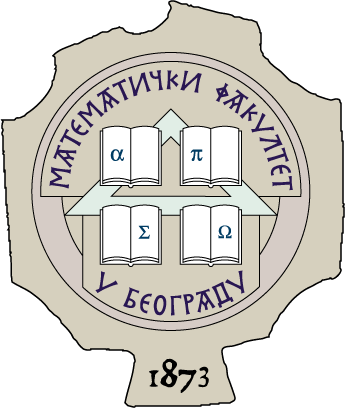
\includegraphics[width=0.2\textwidth]{img/matf-logo.png}
	\end{figure}\\[3cm]
	\textbf{\Large МАСТЕР РАД}\\[0.3cm]
	на катедри за \\[0.3cm]
	\textbf{\Large Рачунарство и информатику}\\[.7cm] % Minor heading such as course title
	на тему\\[0.7cm]
	
	\HRule \\[0.4cm]
	{ \huge \bfseries Примена неуронских поља зрачења у рендеровању}\\[0.4cm] % Title of your document
	\HRule \\[1.5cm]
	
	\begin{minipage}{0.4\textwidth}
		\begin{center}
			Коста Грујчић
		\end{center}
	\end{minipage}\\[5cm]
	
	{\large Београд, \today}\\[2.5cm]
	\vfill
\end{titlepage}
\pagenumbering{roman}

% Defines mentor & date
\newpage
\thispagestyle{empty}

\hspace{0pt}
\vfill
\noindent \textbf{Ментор}:\\
проф. др Младен Николић\\Универзитет у Београду, Математички факултет
\\[2cm]

\noindent \textbf{Чланови комисије}:
\\проф. др Младен Николић\\Универзитет у Београду, Математички факултет
\\[0.25cm]
\\проф. др Младен Николић\\Универзитет у Београду, Математички факултет
\\[0.25cm]
\\проф. др Младен Николић\\Универзитет у Београду, Математички факултет
\\[2cm]

\noindent \textbf{Датум одбране}: \today
\hspace{0pt}
\vfill

\newpage
\thispagestyle{empty}
Посвета

\newpage
\thispagestyle{empty}
\noindent \textbf{Наслов мастер рада}: Примена неуронских поља зрачења у рендеровању

\noindent \textbf{Резиме}:

\noindent \textbf{Кључне речи}: машинско учење, неуронска поља, рендеровање

\listoffigures
\listoftables
\tableofcontents

\pagenumbering{arabic}
\chapter{Увод}
\lipsum[1-20]

\chapter{Основни појмови рачунарске графике}
\section{Светлост и боја}
Светлост представља електромагнетно зрачење чија је таласна дужина у сегменту од око 350 до
700 nm, које побуђује визуелни систем човека. То значи да људи \textit{не виде} светлост
осталих таласних дужина, тако да ћемо убудуће под видљивим спектром светлости мислити управо
на овај, видљив човеку.

%Светлост коју наш визуелни систем региструје мора доћи од неког извора. Тако и разликујемо
%примарне и секундарне изворе светлости, односно изворе који производе зрачење и оне који их
%само рефлектују. Када је реч о рефлексији светлости, она може бити спекуларна када се светлост
%рефлектује дуж тачно једног правца, или дифузна када се расипа.

Потребно је увести физичке величине којима се могу квантификовати основна физичка својства
светлости. Прво ћемо дефинисати радиометријске величине, а онда одговарајуће фотометријске.

\begin{definition}
	Фотон је квант електромагнетног зрачења. Енергија фотона је:
	$$E=\frac{hc}{\lambda},$$ где је $h$ Планкова константа, $c$ брзина светлотси, а $\lambda$ 
	таласна дужина фотона.
\end{definition}

\begin{definition}
	Укупна енергија зрачења извора зрачења је: $$Q_e = \int_{\Omega} E d\omega \left[J\right].$$
\end{definition}

\begin{definition}
	Флукс зрачења је укупна енергија зрачења по једини времена:
	$$\Phi = \frac{\partial Q_e}{\partial t} \left[W\right].$$
\end{definition}

\begin{definition}
	Озраченост је укупан флукс зрачења по једини површине:
	$$E = \frac{\partial \Phi}{\partial A} \left[\frac{W}{m^2}\right].$$
\end{definition}

\begin{definition}
	Јачина зрачења је укупан флукс зрачења по јединичном просторном углу:
	$$I = \frac{\partial \Phi}{\partial \Omega} \left[\frac{W}{sr}\right].$$
\end{definition}

\begin{definition}
	Зрачење је је укупан флукс зрачења по једини површине и јединичном просторном углу:
	$$I = \frac{\partial^2 \Phi}{\partial \Omega \partial A} \left[\frac{W}{sr \cdot m^2}\right].$$
\end{definition}

Фотометријске величине су аналогони радиометријских и даћемо их у поређењу са
радиометријским величинама табелом \ref{table-radio-vs-photo}.

\begin{table}[h]
	\centering
	\begin{tabular}{|l|l|}
		\hline
		{\textbf{Радиометријске величине}} & {\textbf{Фотометријске величине}}\\
		\hline
		{Флукс зрачења $\left[W\right]$} & {Светлосни флукс $\left[lm\right]$} \\ 
		\hline
		{Озраченост $\left[\frac{W}{m^2}\right]$} & {Осветљеност $\left[lx\right]$} \\
		\hline
		{Јачина зрачења $	\left[\frac{W}{sr}\right]$} & {Јачина светлости $\left[cd\right]$} \\
		\hline
		{Зрачење $\left[\frac{W}{sr \cdot m^2}\right]$} & {Сјајност $\left[\frac{cd}{m^2}\right]$}\\
		\hline
	\end{tabular}
	\caption{Поређење радиометријских и фотометријских величина}
	\label{table-radio-vs-photo}
\end{table}

\section{Камера}
	\begin{theorem}
		Неки текст теореме.
	\end{theorem}
	\begin{proof}
		Доказ теореме.
	\end{proof}
	\begin{definition}
		Неки текст дефиниције.
	\end{definition}
	\begin{equation}
		\int_{-\infty}^{\infty}f(t)dt
	\end{equation}
\section{Рендеровање}

\chapter{Основни појмови машинског учења}
У овој глави ћемо формулисати теоријски оквир неопходан за разматрање и примену машинског учења.

Машинско учење је област \textit{вештачке интелигенције}. Неформално говорећи, машинско учење
обухвата алгоритме изведене из података или како се то често говори - научених из података.
То значи да нема експлицитног програмирања, а врло често ни контроле процеса учења, већ се
алгоритми дефинишу низом операција параметризованих на основу података који су изложени
процесу обучавања. Процес обучавања, дакле, представља одређивање поменутих параметара
којима се операције од значаја израчунавају на што исправнији начин. Приметимо да је та
исправност прилично неодређен појам и зависи од примене, података и циља обучавања. Такође,
врло се често не може ни квантификовати што проблем обучавања чини утолико тежим.

Имајући у виду досег овог рада, потребно је увести појам надгледаног учења. Реч је о врсти
учења у којој су уз податке присутни и додатни подаци којима је директно могуће утврдити
да ли је излаз алгоритма исправан или није. На пример, ако је потребно утврдити да ли је на
датој слици мачка, уз слику би постојао једнобитни податак који то недвосмислено потврђује.
Према томе, скуп података можемо посматрати као скуп одбирака $\mathcal{D}=\{x_i, y_i\}$,
где $x_i$ представља улаз, а $y_i$ oдговарајући излаз. То нам омогућава да посматрамо
расподелу таквих одбирака, односно густину расподеле $p(x, y)$. Природно се намеће потреба
за што приближнијем одређивању поменуте расподеле, што подразумева одређивање функције $f$
којом успостављамо везу између одговарајућих парова $x$ и $y$. Кандидата за $f$ има
несагледиво много, а нама је потребна она \textit{најбоља}, при чему се овог пута то мора
формално дефинисати.

Претпоставимо да су $y_i$ узорковани из метричког простора. Зато можемо дефинисати
\textit{функцију грешке} $\mathcal{L}$ којом меримо квалитет апроксимације $y_i$
вредношћу $f(x_i)$. Вреднујући одбирке у складу са својом густином дефинишемо \textit{ризик}
\begin{equation}
	R(f) = \mathbb{E}(\mathcal{L}(y, f(x)))=\int\mathcal{L}(y, f(x))p(x, y)dxy.
	\label{eqn-risk}
\end{equation}

Проблем надгледаног учења покушава да дође до $f$ за које се ризик минимизује. Начелно,
обучавање се може извести по свим могућим функцијама $f$. Како је то практично немогуће,
претрага функција се усмерава увођењем додатних претпоставки, односно рестрикција, скупа
претраге. Ми ћемо посматрати функције параметризоване скупом параметара $\theta$,
тако да минимизовање ризика посматрамо као
\begin{equation}
	\min_{\theta}R(f_{\theta}).
	\label{eqn-min-risk-theta}
\end{equation}
У општем случају nе мора постојати само један исправан излаз за конкретан улаз, што оправдава
дефинисање ризика коришћењем заједничке расподеле $p(x, y)$. То за наше потребе неће бити
неопходно. Наиме, посматраћемо условну расподелу $p(y\vert x)$.

Расподела $p(y\vert x)$ је ретко кад позната. Зато се спроводи стандардни статистички
третман - ризик се мења емпиријским ризиком:
\begin{equation}
	ER(f_\theta, \mathcal{D}) = \frac{1}{\vert \mathcal{S}\vert}\sum_{i=1}^{\vert \mathcal{S}\vert}\mathcal{L}(y_i, f_\theta(x_i)),
\end{equation}
где је $\mathcal{S}$ узорак скупа $\mathcal{D}$.

Претпоставимо да се скуп параметара састоји од само једног вектора димензије свега $2$,
тј. $\theta = \{\mathbf{w}\} = \{(w_1, w_2)\}$,
а да је $x_i \in \mathbb{R}^{1}$. Имајући у виду израз \ref{eqn-min-risk-theta}, за кандидате
функције $f$, између осталог, имамо $\sin(x_i w_1 + w_2)$, $\log(x_i w_1 w_2)$,
$\exp(w_2x_i^{w_1})$. Иако је проблем постављен као веома једноставан, а параметарском
рестрикцијом начињен још једноставнијим, и даље се чини као веома тежак будући да немамо
начин да за разумно коначно времена претражимо све такве кандидате. Зато је потребно посматрати
тачно одређене класе функција $f$ за које је то могуће, а међу најпознатијим су свакако
\textit{неуронске мреже}. Заправо, потребно је фиксирати конкретну архитектуру модела, а
потом вршити оптимизацију параметара у складу са одабраном метриком.

\section{Неуронске мреже}
%Неуронске мреже ћемо дефинисати са пробабилистичког становишта, а то значи да ћемо прво кренути од
%rегресионих модела.
%
%Уколико желимо да моделујемо зависност $\mathbf{w}$ и $\mathbf{x}$, природно је кренути од
%оног најпростијег случаја - линеарног. Зато посматрамо функцију облика
%$$y(\mathbf{x}) = \mathbf{w}^{T}\mathbf{x} + \epsilon = \sum_{j}x_jw_j + \epsilon,$$ при чему се
%димензије вектора параметара $\mathbf{w}$ и улаза $\mathbf{x}$ слажу. Параметар $\epsilon$
%називамо \textbf{резидуалом}. Како је расподела резидуала готово увек непозната, често се
%претпоставља њена нормалност. Тако долазимо до
%$p(y\vert x) = \mathcal{N}(\mathbf{w}^{T}\mathbf{x}, \sigma^2)$.
%Тиме је дефинисан модел \textbf{линеарне регресије}.
%
%У случају када $y$ има само две могуће вредности, има смисла моделовати расподелу $p(y\vert x)$
%Бернулијевом. Тако добијамо $p(y\vert x)=\text{Ber}(y\vert S(\mathbf{w}^T \cdot \mathbf{x}))$,
%где је $S$ сигмоиидна функција\footnote{$S(x) = \frac{1}{1 + \exp(-x)}$}. Тиме је дефинисан
%модел \textbf{логистичке регресије}.

\begin{definition}
	Неуронска мрежа је функција облика
	$$f_{\theta}(\mathbf{x}) = \left(\prod_{i=1}^{L}a_i(\beta_i + W_i)\right) (x),$$
	где је $\theta = \{W_i\}_{i=1}^{L}$ скуп параметара који се обучава,
	$W_i \in \mathbb{R}^{d_i \times d_{i-1}}$ при чему је $d_0 = \dim(x)$ и
	$\{a_i\}_{i=1}^{L}$ функције које се примењују члан по члан. Функције
	$\{a_i\}_{i=1}^{L}$ naзивамо \textbf{активационим функцијама}.
	Параметар $L$ називамо \textbf{бројем слојева неуронске мреже}.
\end{definition}
Активационе функције могу бити произвољне, докле год поштују услове димензионалности. Међутим,
уколико су оне линеарне, тада неуронска мрежа постаје линеарна, односно постаје линеарна регресија.
У циљу добијања што разноврснијих модела, за функције активације се узимају нелинеарне функције.
Један од популарних избора је $ReLU(x) = \max\{0, x\}$ \cite{relu}.

Неуронске мреже су познате и под именом \textit{вишеслојни перцептрони}, па ће убудуће бити
коришћена и скраћеница MLP (eнг. \textit{multilayer perceptron}).

Значајан теоријски резултат даје следећа теорема \cite{universal-approx}
\begin{theorem}
	За сваку функцију $F:\mathbb{R}^n \rightarrow \mathbb{R}^m$ интеграбилну у Бохнеровом смислу
	и свако $\epsilon > 0$, постоји неуронска мрежа $f_\theta$ са ReLU активационим функцијама,
	тако да је $\{d_i=\max\{ n + 1, m\}\}_{i=1}^{L}$ и важи
	$$\int_{\mathbb{R}^n}\left\Vert f_\theta(x) - F(x) \right\Vert dx < \epsilon.$$
\end{theorem}
Ово за последицу има да се готово свака функција може произвољно добро апроксимирати неуронском
мрежом, али како доказ није конструктиван није очигледно како таква неуронска мрежа изгледа.

Уколико су активационе функције диференцијабилне функције, то ће бити и неуронска мрежа. Зато се
поступак минимизације емпиријског ризика спроводи градијентним спустом. Поступак се спроводи у
две етапе - прво се неуронска мрежа примени над подацима пропагацијом унапред, а потом се
пропагацијом уназад користећи правило ланца изврши ажурирање параметара.

Како је градијентни спуст
оптимизација првог реда, није гарантовано да ће пронађени локални минимум бити и глобални. У пракси
се показује да градијентни спуст даје веома добра решења.

Када је реч о имплементацији неуронских мрежа и конкретим детаљима њиховог обучавања, важно је
разматрати хардверска ограничења. Наиме, ови модели могу бити веома комплексни где се ред величине
броја параметара креће и до неколико милиона, па чак и до неколико милијарди. Зато се приликом
обучавања прибегава разнородним техникама, често нумеричке или хеуристичке природе, којима се
смањује укупно време обучавања или смањује утрошак меморије. Еклатантан пример је \textit{стохастички
градијентни спус}т \cite{sgd} - параметри се ажурирају на основу само једног одбирка уместо целог
скупа података. Овај метод је сушта супротност конвенционалном градијентном спусту, тако да се
углавном врши компромис.

\chapter{Неуронска поља зрачења}
\section{NeRF}
\lipsum[1-10]
\section{Mip-NeRF}
\lipsum{1-10}
\section{Instant-NGP}
\lipsum[1-10]

\chapter{Скупови података}
\lipsum[1-20]

\chapter{Експерименти}
\section{Време обучавања}
\section{Квалитет резултата}

\chapter{Закључак}

\bibliographystyle{ieeetr}
\bibliography{refs}
\end{document}
